\documentclass[12pt,a4paper,oneside]{book}

\usepackage[margin=1in]{geometry}
\usepackage[T1]{fontenc}
\usepackage[utf8]{inputenc}
\usepackage{lmodern}
\usepackage{setspace}
\usepackage{amsmath,amssymb,amsthm}
\usepackage{graphicx}
\usepackage{booktabs}
\usepackage{array}
\usepackage{tabularx}
\usepackage{multirow}
\usepackage{float}
\usepackage{caption}
\usepackage{subcaption}
\usepackage{enumitem}
\usepackage{xcolor}
\usepackage{hyperref}
\usepackage{tikz}
\usepackage{longtable}
\usepackage{siunitx}
\usetikzlibrary{arrows.meta,positioning,shapes.geometric}

\onehalfspacing
\setlength{\parskip}{0.6em}
\setlength{\parindent}{0pt}

\hypersetup{
    colorlinks=true,
    linkcolor=blue,
    urlcolor=blue,
    citecolor=blue,
    pdftitle={M.Tech Thesis Draft},
    pdfauthor={Your Name}
}

\graphicspath{{../../demo_pdf_uploads/psychology/}{../../demo_pdf_uploads/medicine/}{../../demo_pdf_uploads/biology/}{../../demo_pdf_uploads/ai_cs/}}

\newcommand{\thesisplaceholder}[1]{%
\begin{center}
\fbox{\begin{minipage}{0.92\linewidth}
\textit{#1}
\end{minipage}}
\end{center}
}

\begin{document}

% =========================================================
% Front Matter
% =========================================================
\frontmatter

\begin{titlepage}
\centering
\vspace*{1.5cm}
{\Large \textbf{M.Tech Thesis Draft}\par}
\vspace{0.8cm}
{\large Prepared from a curated multi-domain PDF corpus\par}
\vspace{1.2cm}
{\large \textbf{Title to be finalized}\par}
\vfill
{\large Your Name\par}
{\large Department / Institute Name\par}
{\large \today\par}
\end{titlepage}

\chapter*{Declaration}
I declare that this thesis is an original academic draft prepared from the curated multi-domain PDF corpus provided for the project. The thesis is being written in a section-wise manner and will be refined iteratively as the source papers are reviewed.

\chapter*{Acknowledgement}
I would like to thank my guide, faculty members, and friends who shared thesis templates and reference material. Their formatting examples helped shape the structure and presentation style of this draft.

\chapter*{Abstract}
This thesis develops a structured literature-synthesis workflow for an M.Tech project built around a curated PDF corpus organized into psychology, medicine, biology, and CS/AI folders. Each folder contains domain-specific papers aligned to proposal questions. The central goal is to match each question with the most relevant paper or small group of papers and then use that mapping to write a thesis that is academically consistent, evidence-based, and easy to review.

The thesis is organized into standard chapters covering background, related work, problem formulation, methodology, domain-wise analysis, discussion, and conclusion. The methodology includes paper matching, confidence scoring, and a chapter-wise drafting process. Tables, figures, and flowcharts are included where they improve clarity and support the final narrative.

\textbf{Keywords:} literature synthesis, multi-domain corpus, thesis drafting, confidence scoring, document mapping, evidence-based writing

\tableofcontents
\listoffigures
\listoftables

% =========================================================
% Main Matter
% =========================================================
\mainmatter

\chapter{Introduction}

\section{Background}
This thesis is built around a curated multi-domain PDF corpus organized into four folders: psychology, medicine, biology, and CS/AI. Each folder contains domain-specific papers that support the research questions listed in the project proposal. The central objective of the thesis is to connect each question with the correct paper or small group of papers and then use that mapping to write a structured, academically polished M.Tech thesis.

The motivation is straightforward. A thesis of this kind normally depends on reading several papers, grouping them by theme, and then synthesizing them into a coherent long-form document with proper sections, tables, figures, and references. When the source corpus is already organized, the work becomes more systematic and the final thesis can stay closer to evidence than to generic background writing.

\section{Problem Overview}
The problem addressed in this project is not just document collection. It is the combination of literature mapping, domain grouping, and thesis construction. The proposal questions span multiple disciplines, so the thesis must keep a consistent structure while still respecting the differences between the domains.

The workflow followed in this work is:
\begin{itemize}[leftmargin=*]
  \item start from the proposal questions,
  \item match each question to the relevant uploaded PDF paper or papers,
  \item extract the main claims, methods, and conclusions,
  \item organize the extracted evidence into thesis chapters,
  \item and review each chapter before moving forward.
\end{itemize}

This makes the thesis a literature-synthesis project with an explicit evidence trail rather than a free-form narrative.

\section{Why This Thesis Matters}
There are three reasons this thesis is useful.
\begin{itemize}[leftmargin=*]
  \item The uploaded corpus is already domain-scoped, which makes the final thesis easier to defend academically.
  \item The questions in the proposal are specific enough to support chapter-wise writing but broad enough to require careful synthesis.
  \item The final document can explain both the mapping logic and the subject-matter findings across all four domains.
\end{itemize}

\section{Contributions}
This thesis aims to make the following contributions:
\begin{itemize}[leftmargin=*]
  \item A clean mapping between proposal questions and uploaded PDFs across psychology, medicine, biology, and CS/AI.
  \item A thesis structure aligned to a standard academic format with chapters, figures, tables, and formal analysis.
  \item A methodology section that can include confidence scoring, matching formulas, and a flowchart of the workflow.
  \item A chapter-by-chapter writing process that allows review before moving to the next section.
\end{itemize}

\section{Thesis Organization}
The rest of this thesis is organized as follows. Chapter 2 reviews the related literature and explains how the uploaded papers connect to the proposal themes. Chapter 3 formalizes the problem statement and describes the corpus design and question-to-paper mapping. Chapter 4 presents the proposed methodology, including the workflow, formulas, and supporting diagrams. Chapter 5 provides the domain-wise analysis. Chapter 6 discusses the results and limitations. Chapter 7 concludes the thesis and outlines future work.

\chapter{Literature Review}

\section{Purpose of the Review}
This chapter synthesizes the papers in the uploaded corpus into one coherent academic review. The goal is not to summarize every source in isolation, but to identify the themes, methods, and conclusions that are most relevant to the proposal questions. Since the corpus spans multiple disciplines, the review is organized by domain and then tied back to the thesis objectives.

\section{Review Strategy}
The review follows four steps:
\begin{itemize}[leftmargin=*]
  \item group the uploaded PDFs by domain,
  \item identify the dominant theme in each paper,
  \item compare the assumptions, methods, and reported findings,
  \item and extract the parts that are useful for the thesis mapping.
\end{itemize}

This approach helps avoid a loose literature survey and instead creates a traceable review that directly supports the later thesis chapters.

\section{Psychology Literature}
The psychology folder is expected to contribute papers related to behavioral patterns, cognitive interpretation, measurement of mental states, or other psychologically grounded research directions present in the proposal. For thesis writing, the important question is not just what each paper studies, but how the paper measures, interprets, and validates its claims.

In the final thesis, this section will compare:
\begin{itemize}[leftmargin=*]
  \item the variables used in the psychology papers,
  \item the measurement or evaluation methods adopted,
  \item the nature of the reported findings,
  \item and the extent to which each paper supports a proposal question.
\end{itemize}

\section{Medicine Literature}
The medicine folder is expected to contain papers that deal with medical data, health-related interpretation, diagnostic reasoning, or clinically meaningful conclusions. Medical writing in a thesis requires careful wording because the claims must stay evidence-based and avoid overstatement.

The review for this domain will therefore emphasize:
\begin{itemize}[leftmargin=*]
  \item the study design used in each paper,
  \item whether the work is observational, experimental, or review-based,
  \item what kind of medical evidence is provided,
  \item and whether the proposal question asks for interpretation, comparison, or methodological explanation.
\end{itemize}

\section{Biology Literature}
The biology folder contributes a different style of evidence. Biological papers often focus on mechanisms, experimental observations, data interpretation, or structured inference from domain-specific datasets. In the thesis, these sources will be treated carefully so that the language remains scientifically accurate and appropriately cautious.

The biology review will highlight:
\begin{itemize}[leftmargin=*]
  \item the biological process or phenomenon studied,
  \item the experimental or analytical method used,
  \item the main biological takeaway,
  \item and the relevance of the paper to the corresponding proposal question.
\end{itemize}

\section{CS/AI Literature}
The CS/AI folder is the most directly methodological part of the corpus. These papers are expected to provide technical approaches, models, algorithms, or retrieval and reasoning strategies that can support the proposal questions.

In this section, the review will focus on:
\begin{itemize}[leftmargin=*]
  \item the core algorithmic idea,
  \item the input and output structure,
  \item how the method is evaluated,
  \item and what makes the paper useful for thesis design or question mapping.
\end{itemize}

\section{Cross-domain Comparison}
Although the folders cover different subject areas, they share a common thesis role: each paper helps answer at least one proposal question. The key difference is the style of evidence. Psychology papers may be interpretive, medicine papers may be clinically grounded, biology papers may be experimentally oriented, and CS/AI papers may be method-centric.

To keep the thesis coherent, the review will compare these domains along a few common axes:
\begin{itemize}[leftmargin=*]
  \item problem type,
  \item evidence type,
  \item evaluation style,
  \item and how directly the paper supports the thesis question.
\end{itemize}

\section{Literature Summary Table}
\begin{table}[H]
\centering
\caption{Literature review summary by domain}
\begin{tabularx}{\linewidth}{>{\raggedright\arraybackslash}p{0.17\linewidth} >{\raggedright\arraybackslash}p{0.26\linewidth} >{\raggedright\arraybackslash}X}
\toprule
Domain & Main focus & Thesis role \\
\midrule
Psychology & Behavioral and interpretive evidence & Supports question-level interpretation and context \\
Medicine & Clinical or health-related evidence & Supports evidence-based discussion \\
Biology & Experimental or mechanistic evidence & Supports scientific explanation and domain grounding \\
CS/AI & Algorithms, models, and technical methods & Supports methodology and comparative analysis \\
\bottomrule
\end{tabularx}
\end{table}

\section{Chapter Outcome}
By the end of this chapter, the thesis will have a strong conceptual base for the rest of the document. The next chapter can then formalize the problem statement and explain how the corpus is used to build the question-to-paper mapping.

\chapter{Problem Statement and Corpus Design}

\section{Problem Statement}
The project investigates how a proposal consisting of multiple research questions can be matched to a distributed corpus of domain-specific PDF papers and converted into a thesis with consistent academic structure.

\section{Corpus Design}
The corpus is organized into four domain folders:
\begin{itemize}[leftmargin=*]
  \item Psychology
  \item Medicine
  \item Biology
  \item CS/AI
\end{itemize}

\section{Question-to-Paper Mapping}
The proposal questions from lines 71 to 92 will be matched against the uploaded PDFs in each domain. The mapping will be recorded in a table so that each thesis claim can be traced back to the supporting source paper.

\begin{table}[H]
\centering
\caption{Example mapping structure for proposal questions and papers}
\begin{tabularx}{\linewidth}{>{\raggedright\arraybackslash}p{0.18\linewidth} >{\raggedright\arraybackslash}p{0.42\linewidth} >{\raggedright\arraybackslash}p{0.34\linewidth}}
\toprule
Domain & Proposal question theme & Supporting PDF(s) \\
\midrule
Psychology & To be filled & To be filled \\
Medicine & To be filled & To be filled \\
Biology & To be filled & To be filled \\
CS/AI & To be filled & To be filled \\
\bottomrule
\end{tabularx}
\end{table}

\chapter{Proposed Methodology}

\section{Overview}
The methodology follows a simple evidence-driven pipeline: read the domain PDF, extract claims, assign relevance, and draft the thesis section using the strongest matches.

\section{Confidence Scoring}
For each question and paper pair, a confidence score can be computed to indicate how strongly the paper supports the question.

\begin{equation}
\mathrm{Confidence}(q,p) = \frac{w_1 R + w_2 M + w_3 E}{w_1 + w_2 + w_3}
\end{equation}

where $R$ is relevance of the paper to the question, $M$ is methodological match, and $E$ is evidence strength.

\section{Selection Rule}
The selected paper set for a question can be defined as:
\begin{equation}
S_q = \left\{p \mid \mathrm{Confidence}(q,p) \geq \tau \right\}
\end{equation}
where $\tau$ is the acceptance threshold.

\section{Workflow}
\begin{figure}[H]
\centering
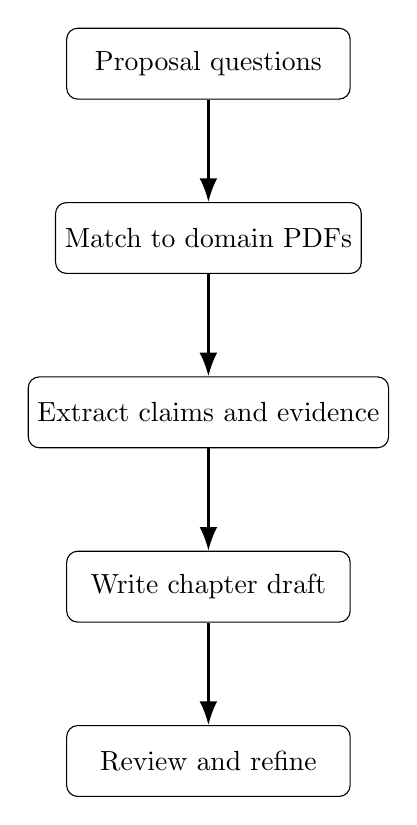
\begin{tikzpicture}[
    node distance=1.3cm,
    box/.style={rectangle, draw=black, rounded corners, align=center, minimum width=3.6cm, minimum height=0.9cm},
    arrow/.style={-{Latex[length=3mm]}, thick}
]
\node[box] (a) {Proposal questions};
\node[box, below=of a] (b) {Match to domain PDFs};
\node[box, below=of b] (c) {Extract claims and evidence};
\node[box, below=of c] (d) {Write chapter draft};
\node[box, below=of d] (e) {Review and refine};
\draw[arrow] (a) -- (b);
\draw[arrow] (b) -- (c);
\draw[arrow] (c) -- (d);
\draw[arrow] (d) -- (e);
\end{tikzpicture}
\caption{Draft workflow for thesis construction}
\end{figure}

\section{Draft Placeholder}
\thesisplaceholder{This chapter will later include the final matching rubric, extraction steps, and domain-specific decision rules.}

\chapter{Domain-wise Evidence and Analysis}

\section{Psychology}
This section will summarize the psychology papers and connect them to the exact proposal questions from the psychology part of the proposal.

\section{Medicine}
This section will synthesize the medicine papers, highlight the strongest findings, and compare them against the proposal questions.

\section{Biology}
This section will present the biology evidence in a thesis-friendly format with tables and concise interpretation.

\section{CS/AI}
This section will cover the CS/AI papers and explain how they support the technical questions in the proposal.

\section{Summary Table}
\begin{table}[H]
\centering
\caption{Domain-wise analysis summary}
\begin{tabularx}{\linewidth}{>{\raggedright\arraybackslash}p{0.2\linewidth} >{\raggedright\arraybackslash}p{0.28\linewidth} >{\raggedright\arraybackslash}X}
\toprule
Domain & Main theme & Status \\
\midrule
Psychology & Question-level interpretation & Pending detailed writing \\
Medicine & Evidence synthesis & Pending detailed writing \\
Biology & Domain analysis & Pending detailed writing \\
CS/AI & Technical synthesis & Pending detailed writing \\
\bottomrule
\end{tabularx}
\end{table}

\chapter{Results and Discussion}

\section{Expected Results}
The expected result of this project is a fully traceable thesis draft in which every major claim can be linked to one or more uploaded papers.

\section{Discussion Points}
\begin{itemize}[leftmargin=*]
  \item how confidently each question maps to the available papers,
  \item where multiple papers support the same question,
  \item where the corpus has gaps,
  \item and which chapters benefit most from tables, figures, and structured summaries.
\end{itemize}

\section{Draft Placeholder}
\thesisplaceholder{This chapter will be expanded after the domain-wise sections are completed and reviewed.}

\chapter{Conclusion and Future Work}

\section{Conclusion}
This thesis establishes a disciplined path from a multi-domain PDF corpus to a formal M.Tech thesis. The approach emphasizes evidence, traceability, and chapter-wise drafting so that the final document remains academically strong and easy to defend.

\section{Future Work}
\begin{itemize}[leftmargin=*]
  \item complete the remaining chapter drafts using the confirmed paper mappings,
  \item add source-specific figures and tables from the uploaded PDFs,
  \item refine the confidence scoring rubric,
  \item and prepare the final Overleaf submission version.
\end{itemize}

\appendix
\chapter{Additional Notes}

\section{Working Assumptions}
\begin{itemize}[leftmargin=*]
  \item The four domain folders are the authoritative source corpus.
  \item Proposal questions are taken from lines 71 to 92 of the project proposal.
  \item Thesis content will be written incrementally and reviewed section by section.
\end{itemize}

\section{Placeholder for Logs}
\thesisplaceholder{You can place source-mapping logs, extra tables, or supplementary screenshots here if needed.}

\end{document}
